\documentclass[10.5pt,notitlepage]{article}
\usepackage[utf8]{inputenc}
\usepackage{amsthm}
\usepackage{amsmath}
\usepackage{amsfonts}
\usepackage{mathtools}
\usepackage{amsmath,amssymb}       
\usepackage{enumitem}   
\usepackage{enumerate}
\usepackage{graphicx}
\usepackage{bbm}
\usepackage{booktabs}
\renewcommand{\qedsymbol}{$\blacksquare$}
\usepackage{makecell}
\usepackage[spanish]{babel}
\decimalpoint
\usepackage[letterpaper]{geometry}
\graphicspath{ {images/} }
\usepackage{mathrsfs}
\newenvironment{solucion}
  {\begin{proof}[Solución]}
  {\end{proof}}
\pagestyle{plain}
\usepackage{pdflscape}
\usepackage[table, dvipsnames]{xcolor}
\usepackage{longtable}
\usepackage{tikz}
\def\checkmark{\tikz\fill[scale=0.4](0,.35) -- (.25,0) -- (1,.7) -- (.25,.15) -- cycle;} 
\usepackage[bottom]{footmisc}
\usepackage{hyperref}
\usepackage{float}
\usepackage[utf8]{inputenc}
\usepackage{bbm}
\usepackage{placeins}
\newcommand{\pp}{\mathbb{P}}
\newcommand{\BB}{\mathcal{B}}
\newcommand{\RR}{\mathbb{R}}
\newcommand{\FF}{\mathcal{F}}
\newcommand{\CC}{\mathcal{C}}
\newcommand{\AA}{\mathcal{A}}
\newcommand{\oo}{\varnothing}
\newcommand{\ee}{\varepsilon}
\newcommand{\NN}{\mathbb{N}}
\newcommand{\PP}{\mathcal{P}}
\newcommand{\LL}{\mathrm{L}}
\newcommand{\XX}{\mathbf{X}}
\newcommand{\xx}{\mathcal{X}}
\newcommand{\abs}[1]{\left\lvert #1 \right\rvert}
\newcommand{\norm}[1]{\left\| #1 \right\|}
\newcommand{\inner}[1]{\left\langle #1 \right\rangle}
\newcommand{\corch}[1]{\left[ #1 \right]}
\newcommand{\kis}[1]{\left\{ #1 \right\}}
\newcommand{\pare}[1]{\left( #1 \right)}



\title{Tarea 2: Modelos Estadísticos I.}

\author{Rojas Gutiérrez Rodolfo Emmanuel}
\date{\today}


\begin{document}

\maketitle

\section{Ejercicios.}


\noindent \textbf{Ejercicio 1.} \textbf{(a)} Pruebe que las estimaciones de mínimo cuadráticas \(a_1,\hdots,a_m,b\) de los parámetros \(\alpha_1,\hdots,\alpha_m,\beta\) de la familia de rectas 
\[
E[Y_i] = \alpha_i+\beta X_i, \ i = 1,\hdots,m,
\]
están dados por 
\begin{align}
    b &= \frac{\sum_{i = 1}^{m}\sum_{j=1}^{n_i}(X_{ij} - \overline{X_i})(Y_{ij} - \overline{Y_i})}{\sum_{i = 1}^{m}\sum_{j=1}^{n_i}(X_{ij} - \overline{X_i})^2}, \label{1.-1}\\ 
    a_i &= \overline{Y}_i - b \overline{X}_i, \label{1.0},
\end{align}
donde \((X_{i1},Y_{i1}),\hdots,(X_{in_i},Y_{in_i})\) denotan los valores observados de \((X_i,Y_i)\) relacionados con la \(i\)-ésima recta, \(i = 1,\hdots, m\).\\

\noindent\textbf{(b)} Pruebe que la suma de cuadrados residual está dada por 
\begin{equation}\label{1.1}
    S^2 = \sum_{i = 1}^{m}\sum_{j=1}^{n_i}(Y_{ij} - \overline{Y_i}) - b^2 \sum_{i = 1}^{m}\sum_{j=1}^{n_i}(X_{ij} - \overline{X_i})^2,
\end{equation}
con \(\sum_{i = 1}^{m}n_i - m -1\) grados de libertad.
\begin{solucion}
\noindent\textbf{(a)} Sea \((X_{11},Y_{11}),\hdots,(X_{1n_1},Y_{1n_1}), \hdots, (X_{m1},Y_{m1}),\hdots,(X_{mn_m},Y_{mn_m})\) una muestra observada, donde \((X_{i1},Y_{i1}),\hdots,(X_{in_i},Y_{in_i})\) denotan los valores observados de \((X_i,Y_i)\) relacionados con la \(i\)-ésima recta, \(i = 1,\hdots, m\). Defina para \(i \in \{1,\hdots,m\}\)
\begin{equation*}
     \overline{Y}_i &= \frac{1}{n_i}\sum_{j = 1}^{n_i}Y_{ij},\ \ \overline{X}_i &= \frac{1}{n_i}\sum_{j = 1}^{n_i}X_{ij},
\end{equation*}
entonces se cumple para cada \(i \in \{1, \hdots, m\}\)
\begin{align}
    \sum_{j = 1}^{n_i}(Y_{ij} - \overline{Y}_i)^2 &= \sum_{j = 1}^{n_i}Y_{ij}^2 - n_i \overline{Y}_{i}^{2}, \label{1.2}\\ 
    \sum_{j = 1}^{n_i}(X_{ij} - \overline{X}_i)^2 &= \sum_{j = 1}^{n_i}X_{ij}^2 - n_i \overline{X}_{i}^{2}, \label{1.3}\\ 
    \sum_{j = 1}^{n_i}(X_{ij} - \overline{X}_i)(Y_{ij} - \overline{Y}_i) &= \sum_{j = 1}^{n_i}X_{ij}Y_{ij} - n_i \overline{X}_i \overline{Y}_i, \label{1.4}
\end{align}
lo anterior servirá a lo largo de la prueba. Como se desea obtener las estimaciones por mínimos cuadrados de los parámetros \(\alpha_1,\hdots,\alpha_m, \beta\) entonces se intentará minimizar la función \(f:\mathbb{R}^{m+1} \to \RR^{+}\) con regla de correspondencia 
\begin{equation}\label{1.5}
    f(a_1,\hdots,a_m,b) = \sum_{i=1}^{m}\sum_{j=1}^{n_i}(Y_{ij} - a_i - bX_{ij})^2, 
\end{equation}
para ello se buscará el punto en el que \(\nabla f = 0\). Con esto en mente observe que para cada \(r \in \{1,\hdots,m\}\) se satisface que 
\begin{equation}\label{1.6}
    \frac{\partial f}{\partial a_r} = -2\sum_{j = 1}^{n_r}(Y_{rj} - a_r - b X_{rj}),
\end{equation}
por otro lado, note que 
\begin{equation}\label{1.7}
    \frac{\partial f}{\partial b} = -2\sum_{i = 1}^{m}\sum_{j=1}^{n_i}X_{ij}\corch{Y_{ij} - a_i - bX_{ij}},   
\end{equation}
igualando las expresiones en (\ref{1.6}) a cero obtenemos que 
\begin{align}
     0 =  \frac{\partial f}{\partial a_r} &\iff  \sum_{j = 1}^{n_r}(Y_{rj} - a_r - b X_{rj}) = 0,\nonumber\\ 
     -n_r a_r + n_r \overline{Y}_r - b n_r\overline{X}_r =0 &\iff a_r = \overline{Y}_r - b\overline{X}_r, \label{1.8} 
\end{align}
por otra parte, igualando la expresión (\ref{1.7}) a cero y multiplicando por \(- \frac{1}{2}\) la desigualdad resultante se obtiene 
\begin{align}
    0 &= \sum_{i = 1}^{m}\sum_{j=1}^{n_i}X_{ij}\corch{Y_{ij} - a_i - bX_{ij}} = \sum_{i = 1}^{m}\corch{\sum_{j=1}^{n_i}X_{ij}Y_{ij} - a_in_i\overline{X}_i - b\sum_{j = 1}^{n_i}X_{ij}^2} \nonumber\\ 
      &\textbf{Usando (\ref{1.8}) para sustituir el termino \(a_i\) se obtiene que.}\nonumber\\
      &=\sum_{i = 1}^{m}\corch{\sum_{j=1}^{n_i}X_{ij}Y_{ij} - n_i\pare{\overline{Y}_i - b\overline{X}_i}\overline{X}_i - b\sum_{j = 1}^{n_i}X_{ij}^2} \nonumber\\ 
      &=\sum_{i = 1}^{m}\corch{\sum_{j=1}^{n_i}X_{ij}Y_{ij} -n_i\overline{X}_i\overline{Y}_i - b\pare{\sum_{j = 1}^{n_i}X_{ij}^2 - n_i\overline{X}_{i}^{2}} } = (*)\nonumber
\end{align}  
\begin{align}
     (*) &=\underbrace{\sum_{i = 1}^{m}\corch{\sum_{j = 1}^{n_i}(X_{ij} - \overline{X}_i)(Y_{ij} - \overline{Y}_i) - b\sum_{j = 1}^{n_i}(X_{ij} - \overline{X}_i)^2 }}_{\text{Por (\ref{1.3}) y (\ref{1.4}).}}\nonumber\\ 
\end{align}
de este modo 
\[
\sum_{i = 1}^{m}\corch{\sum_{j = 1}^{n_i}(X_{ij} - \overline{X}_i)(Y_{ij} - \overline{Y}_i) - b\sum_{j = 1}^{n_i}(X_{ij} - \overline{X}_i)^2 } = 0,
\]
así pues
\begin{equation}\label{1.9}
    b = \frac{\sum_{i=1}^{m}\sum_{j = 1}^{n_i}(X_{ij} - \overline{X}_i)(Y_{ij} - \overline{Y}_i)}{\sum_{i=1}^{m}\sum_{j = 1}^{n_i}(X_{ij} - \overline{X}_i)^2},
\end{equation}
y de (\ref{1.8}) se tenía que 
\[
  a_r = \overline{Y}_r - b\overline{X}_r, \ r\in\{1,\hdots,m\}. 
\]
por ende, la solución a \(\nabla f = 0\) es precisamente la expresada anteriormente, y lo anterior son los estimadores por mínimos cuadrados de los interceptos y el parámetro de pendiente. \\ 

\noindent \textbf{(b)} Observe que los residuales en este caso están dados por 
\[
e_{ij} = Y_{ij} - a_i - bX_{ij}, \ \text{ con \(i=\{1,\hdots,m\}\) y \(j = \{1,\hdots,n_i\}\),}
\]
de este modo la suma de cuadrados residuales \(S^2\) esta dada por 
\begin{align}
    S^2 &= \sum_{i = 1}^{m}\sum_{j = 1}^{n_i}e_{ij}^2 = \sum_{i = 1}^{m}\sum_{j = 1}^{n_i}\pare{Y_{ij} - a_i - bX_{ij}}^2 \nonumber\\
        &\textbf{Usando (\ref{1.8}) para sustituir el termino \(a_i\) se obtiene que.}\nonumber\\
        &= \sum_{i = 1}^{m}\sum_{j = 1}^{n_i}\pare{Y_{ij} - \overline{Y}_i -b(X_{ij} - \overline{X}_i)}^2. \label{1.10}
\end{align}
Por otro lado observe que de (\ref{1.9}) se sigue que 
\begin{equation}\label{1.11}
     b \sum_{i = 1}^{m}\sum_{j = 1}^{n_i}(X_{ij} - \overline{X}_i)^2 =  \sum_{i = 1}^{m}\sum_{j = 1}^{n_i}(X_{ij} - \overline{X}_i)(Y_{ij} - \overline{Y}_i),
\end{equation}
de este modo
\begin{align}
     \sum_{i = 1}^{m}\sum_{j = 1}^{n_i}\pare{Y_{ij} - \overline{Y}_i -b(X_{ij} - \overline{X}_i)}^2 &=   \sum_{i = 1}^{m}\sum_{j = 1}^{n_i}(Y_{ij} - \overline{Y}_i)^2-2b \sum_{i = 1}^{m}\sum_{j = 1}^{n_i}(Y_{ij} - \overline{Y}_i)(X_{ij} - \overline{X}_i)+b^2 \sum_{i = 1}^{m}\sum_{j = 1}^{n_i}(X_{ij} - \overline{X}_i)^2\nonumber\\ 
    &=   \sum_{i = 1}^{m}\sum_{j = 1}^{n_i}(Y_{ij} - \overline{Y}_i)^2 \underbrace{- 2b^2 \sum_{i = 1}^{m}\sum_{j = 1}^{n_i}(X_{ij} - \overline{X}_i)^2}_{\text{Por (\ref{1.11}).}}+ b^2 \sum_{i = 1}^{m}\sum_{j = 1}^{n_i}(X_{ij} - \overline{X}_i)^2\nonumber\\ 
    &=  \sum_{i = 1}^{m}\sum_{j = 1}^{n_i}(Y_{ij} - \overline{Y}_i)^2 - b^2 \sum_{i = 1}^{m}\sum_{j = 1}^{n_i}(X_{ij} - \overline{X}_i)^2 \label{1.12}, 
\end{align}
de (\ref{1.10}) y (\ref{1.12}) se sigue 
\[
S^2 = \sum_{i = 1}^{m}\sum_{j = 1}^{n_i}(Y_{ij} - \overline{Y}_i)^2 - b^2\sum_{i = 1}^{m}\sum_{j = 1}^{n_i}(X_{ij} - \overline{X}_i)^2,
\]
con \(\sum_{i = 1}^{m}n_i - m -1\) grados de libertad, el número de datos observados menos el número de parámetros a estimar.
\end{solucion}
%%%%%%%%%%%%%%%%%%%%%%%%%%%%%%%%%%%%%%%%%%%%%%%%%%%%%%%%%%%%%%%%%%%%%%%%%%%%%%%%%%%%%%%%%%%%%%%%%%%%%%%%%%%%%%%%%%%%%%%%%%%%%%%%%%%%%%%%%%%%%%%%%%%%%%%%%
\noindent \textbf{Ejercicio 2.} Los datos de la siguiente tabla muestran la relación entre la frecuencia cardiaca en reposo (Y) y el peso corporal en kilogramos \(X\)
\\

\noindent\textbf{(a)} Grafique estos datos. ¿Parece que hay una relación lineal entre el peso corporal y la frecuencia cardiaca en reposo?\\

\noindent\textbf{(b)} Calcule las estimaciones \(\hat{\beta}_0\) y \(\hat{\beta}_1\) y escriba la ecuación de regresión para estos datos. Grafique la línea de regresión sobre la gráfica de dispersión del inciso \textbf{(a)} interprete los coeficientes de regresión estimados. \\

\noindent\textbf{(c)} Ahora examine el punto \((67,40)\). Si dicho punto fuera eliminado del conjunto de datos, ¿qué cambios resultarian en las estimaciones del intercepto y la pendiente?\\

\noindent\textbf{(d)} Obtenga la estimación puntual de la respuesta media cuando \(x = 88\). Obtenga un intervalo de \(95\%\) de confianza para la respuesta media \(X = 88 kg\). Interprete este intervalo.\\

\noindent\textbf{(e)} Pronostique la frecuencia cardiaca para una persona cuyo peso corporal sea de \(88 kg\) utilizando una predicción puntual y una por intervalo del \(95\%\) de confianza. Compare estas predicciones con la estimación del inciso \textbf{(d)}. \\

\noindent\textbf{(f)} Sin hacer cálculos, ¿para que valor medido de \(X\) la correspondiente \(\hat{Y}\) tendría la menor varianza? ¿Por qué?
\begin{solucion}
\noindent\textbf{(a)} La gráfica solicitada se presenta en la figura \ref{fig:RLineal} en la misma se puede decir que no se nota a primer instancia una relación lineal entre las observaciones.
  \begin{figure}[htb]
 \centering
 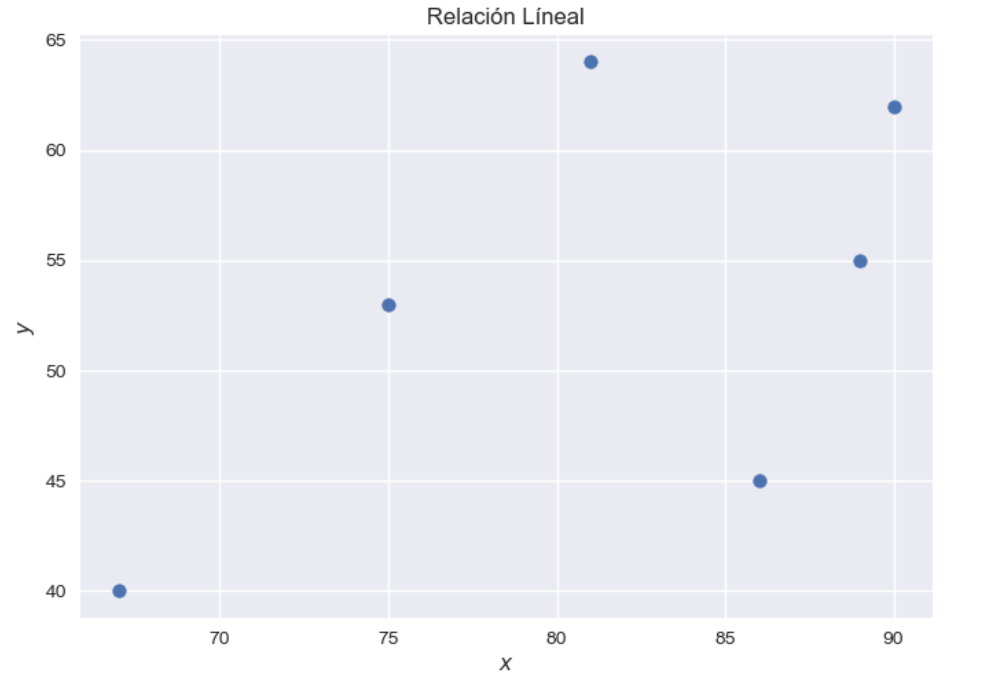
\includegraphics[scale = 0.6]{Relación lineal.png}
 \caption{Relación Lineal.}
 \label{fig:RLineal}
 \end{figure}\\


\noindent\textbf{(b)} Con los datos proporcionados el coeficiente de pendiente puede calcularse como 
\begin{equation}\label{b1}
    \hat{\beta}_1= \frac{\sum_{i=1}^{6}X_iY_i - 6 \overline{X} \overline{Y}}{\sum_{i=1}^{6}X_{i}^2 - 6\overline{x}^2} \approx 0.595,
\end{equation}
por otro lado se sabe que 
\begin{equation}\label{b2}
    \hat{\beta}_0 = \overline{Y} - \hat{\beta}_1\overline{X} \approx 4.799,
\end{equation}
por lo que la ecuación de la recta de regresión esta dada por 
\begin{equation}\label{b3}
   \widehat{E}[Y_i|X_i] = 4.799 +  0.595 X_i,  
\end{equation}
la gráfica de la recta de regresión ajustada sobre los datos puede consultarse en la figura \ref{fig:RLineal2}. Por otro lado podemos interpretar el coeficiente de pendiente \(\hat{\beta}_1\) como el cambio estimado en la media de la frecuencia cardiaca dada una variación de un kilogramo en el peso, por ejemplo si se aumenta un kilo en el peso entonces la frecuencia cardiaca se elevara en \(0.595\) latidos por minuto. Por otra parte, el intercepto puede ser interpretado como la estimación de la media de la frecuencia cardiaca para un nivel de peso de \(0\) kilogramos, pese a ello esta interpretación es un poco inútil dentro del contexto del problema. 
  \begin{figure}[htb]
 \centering
 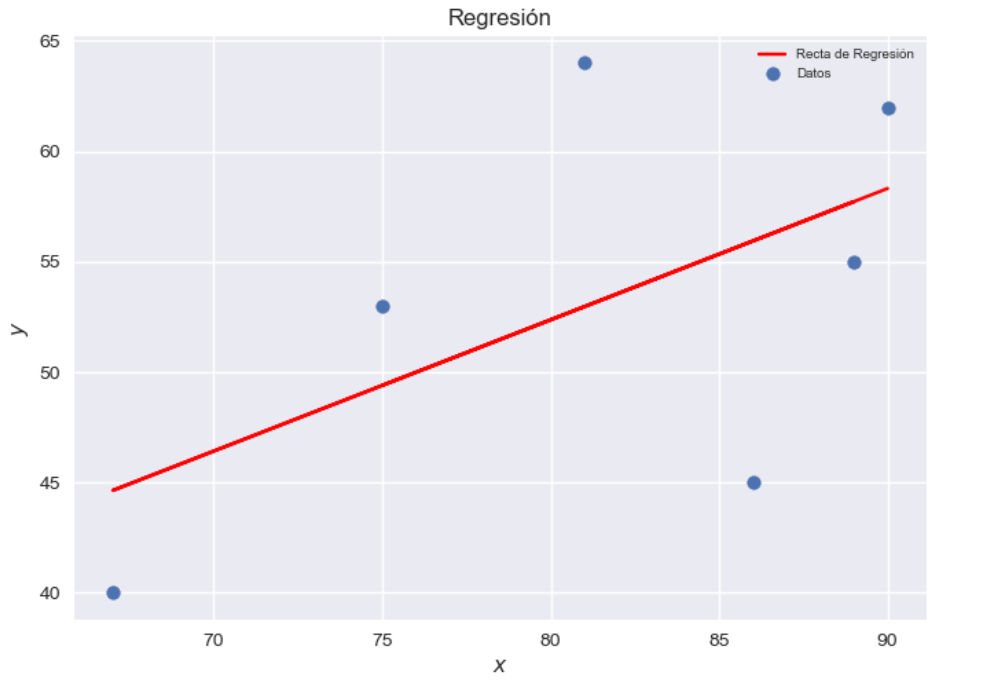
\includegraphics[scale = 0.6]{Relación lineal 2.png}
 \caption{Recta de Regresión Sobre el Conjunto de Datos.}
 \label{fig:RLineal2}
 \end{figure}


\noindent\textbf{(c)} Sí se eliminara el punto \((67,40)\) se tendrían las siguientes estimaciones para \(\beta_1\) y \(\beta_0\)
\begin{equation}\label{b11}
    \hat{\beta}_{1}^{*}= \frac{\sum_{i=1}^{6}X_iY_i -67\cdot 40 - (5)\pare{\frac{\sum X_i - 67}{5}\frac{\sum Y_i - 40}{5}}}{\sum_{i=1}^{6}X_{i}^2- 67^2 - 5\pare{\frac{\sum X_i - 67}{5}} ^2} \approx 0.079, 
\end{equation}
por otro lado, se sabe que 
\begin{equation}\label{b12}
    \hat{\beta}_{0}^{*} = \frac{\sum Y_i - 40}{5} - \hat{\beta}_1\frac{\sum X_i - 67}{5} \approx 49.164,
\end{equation}
por lo que, la ecuación de la recta de regresión en este caso esta dada por 
\begin{equation}\label{b13}
   \widehat{E}[Y_i|X_i] = 49.164 +  0.079 X_i,  
\end{equation}
comparando los estimadores calculados en (\ref{b1}) y (\ref{b2}) con los que fueron calculados en (\ref{b11}) y (\ref{b12}), se puede notar como el intercepto creció bastante y el término de pendiente se hizo mucho más cercano a cero, esto se debe a que si observa con detenimiento la figura \ref{fig:RLineal2} es fácil percatarse que el punto removido es aquel que queda en la esquina inferior izquierda, el mismo parece ser el culpable de que la recta de regresión quede inclinada de esa manera y por ende la pendiente sea mas pronunciada en ese caso. \\ 

\noindent\textbf{(d)} La estimación puntual para la media de la frecuencia cardiaca dado un valor de \(X = 88\) está dada por 
\begin{equation}\label{b4}
     \widehat{E}(Y|X = 88) = \hat{\beta}_0 + \hat{\beta}_1 \cdot 88 \approx 57.131.  
\end{equation}
Con \(\hat{\beta}_1,\hat{\beta}_0\) como en (\ref{b1}) y (\ref{b2}). Mientras que para realizar la estimación por intervalos primero se calculara la cantidad 
\begin{equation}\label{b5}
    s = \sqrt{\frac{SS(Res)}{n-2}} =\sqrt{\frac{\sum_{i=1}^{6}Y_{i}^2 - 6\overline{Y}^2 -\hat{\beta}_{1}^{2}\corch{\sum_{i=1}^{6}X_{i}^2 - 6 \overline{X}^2}}{4}} \approx 8.615.
\end{equation}
Sea \(\alpha = 0.05\) y \(t = t_{4,\frac{\alpha}{2}}\) el cuantil \(\frac{\alpha}{2}\) de una distribución \(t\) con \(4\) grados de libertad entonces el intervalo de confianza del \(95\%\) para la media de la frecuencia cardiaca, dado un nivel del peso de \(88\) kilogramos, esta dado por 
\begin{align}\label{b6}
    &\corch{\widehat{E}(Y|X = 88) + t\cdot s\cdot\sqrt{\frac{1}{6} + \frac{(88 - \overline{X})^2}{\sum_{i=1}X_{i}^{2} - 6\overline{X}^2}}  , \widehat{E}(Y|X = 88) -t\cdot s\cdot\sqrt{\frac{1}{6} + \frac{(88 - \overline{X})^2}{\sum_{i=1}X_{i}^{2} - 6\overline{X}^2}} }\nonumber\\ 
    &= [44.533, 69.730],
\end{align}
recuerde que el intervalo de confianza de \(95\%\) de confianza es un intervalo aleatorio, donde el nivel de confianza hace referencia a que el mismo contiene en un \(95\%\) de las veces al verdadero valor de la media de la respuesta dado un valor de la variable independiente de \(X = 88kg\), por ende con los datos con los que se ajusto el modelo se tendrá con un \(95\%\) de confianza que la media de la frecuencia cardiaca de una persona cuyo peso es de \(88kg\), se encuentra entre \(44.533\) y \( 69.730\) latidos por minuto.   
\\ 

\noindent\textbf{(e)} La estimación puntual para la frecuencia cardiaca dado un valor de \(X = 88\), también conocida como pronóstico o predicción, está nuevamente dada por 
\begin{equation*}
    \hat{Y}_{pred}=\widehat{E}(Y|X = 88)= 88 = \hat{\beta}_0 + \hat{\beta}_1 \cdot 88 \approx 57.131.  
\end{equation*}
Con \(\hat{\beta}_1,\hat{\beta}_0\) como en (\ref{b1}) y (\ref{b2}). Mientras que para calcular los intervalos de predicción se utilizará el estadístico \(s\) (\ref{b5}), y nuevamente sea \(\alpha = 0.05\) y \(t = t_{4,\frac{\alpha}{2}}\) el cuantil \(\frac{\alpha}{2}\) de una distribución \(t\) con \(4\) grados de libertad entonces el intervalo de predicción con confianza del \(95\%\) para la frecuencia cardiaca, dado un nivel del peso de \(88\) kilogramos esta dado por 
\begin{align}\label{b7}
    &\corch{\widehat{E}(Y|X = 88) + t\cdot s\cdot\sqrt{1 + \frac{1}{6} + \frac{(88 - \overline{X})^2}{\sum_{i=1}X_{i}^{2} - 6\overline{X}^2}}  , \widehat{E}(Y|X = 88) -t\cdot s\cdot\sqrt{1+ \frac{1}{6} + \frac{(88 - \overline{X})^2}{\sum_{i=1}X_{i}^{2} - 6\overline{X}^2}} }\nonumber\\ 
    &= [30.096,84.166],
\end{align}
Observe que las estimaciones puntuales son idénticas, mientras que el intervalo de predicción es ligeramente más ancho que el intervalo de confianza, esto se debe a que el valor de la predicción siempre posee un variabilidad mayor a la de su valor promedio.\\ 

\noindent\textbf{(f)} Viendo a \(\hat{Y}\) como estimador de la media de la frecuencia cardíaca para cierto nivel de peso \(X\), observe que la varianza de \(Y\) está dada por 
\[
V(\hat{Y}) = \sqrt{\frac{1}{n} + \frac{(X - \overline{X})}{\sum_{i=1}^n(X_i - \overline{X})^2}} \geq \sqrt{\frac{1}{n}}, 
\]
donde el valor a la derecha se alcanza sí y solo si \(X = \overline{X}\). De igual modo si se toma a \(\hat{Y}\) como predicción de la frecuencia cardiaca para cierto nivel de peso \(X\), se tiene que su varianza está dada por
\[
V(\hat{Y}) = \sqrt{1 + \frac{1}{n} + \frac{(X - \overline{X})}{\sum_{i=1}^n(X_i - \overline{X})^2}} \geq \sqrt{ 1 +\frac{1}{n}}, 
\]
donde el valor a la derecha se alcanza sí y solo si \(X = \overline{X}\). Por lo que, el valor que minimiza la varianza de \(\hat{Y}\) es justamente la media de las \(X_i\).\\ 

Por último en la figura \ref{fig:RLineal3}, se deja una gráfica de la recta de regresión lineal ajustada sobre los datos con los intervalos de predicción y confianza correspondientes. 
\begin{figure}[htb]
\centering
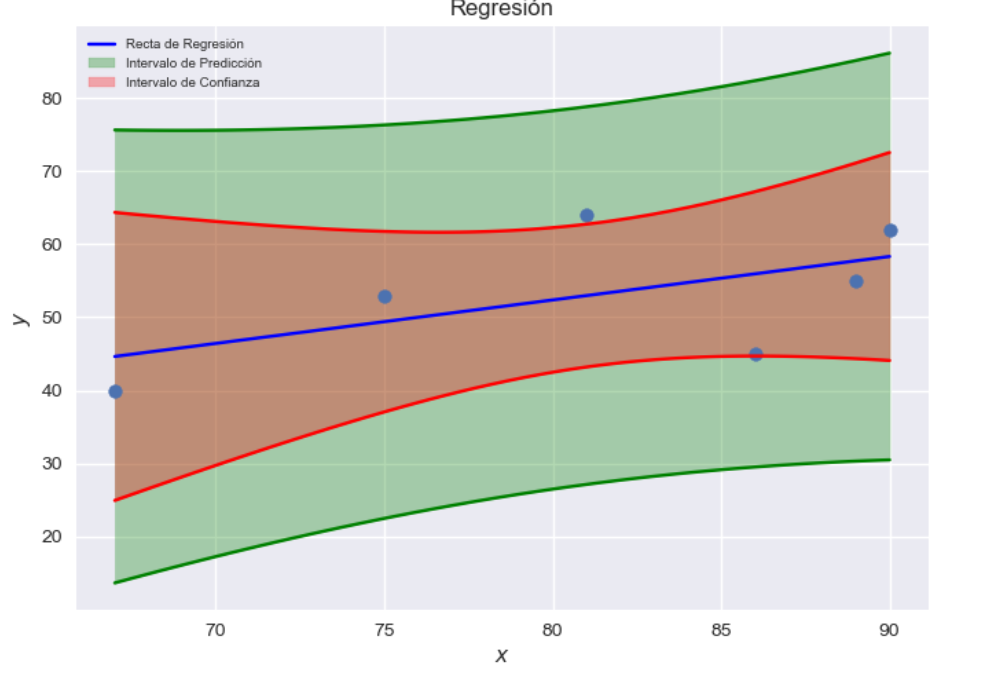
\includegraphics[scale = 0.6]{Relación lineal 3.png}
\caption{Gráfica con intervalos.}
\label{fig:RLineal3}
\end{figure}

\end{solucion}




%%%%%%%%%%%%%%%%%%%%%%%%%%%%%%%%%%%%%%%%%%%%%%%%%%%%%%%%%%%%%%%%%%%%%%%%%%%%%%%%%%%%%%%%%%%%%%%%%%%%%%%%%%%%%%%%%%%%%%%%%%%%%%%%%%%%%%%%%%%%%%%%%%%%%%%%%
\noindent \textbf{Ejercicio 3.} Use los datos del ejercicio 2 y calcule el valor de \(\hat{Y}_i\) para cada valor de \(X\). Calcule las correlaciones entre\\

\noindent\textbf{(a)} \(X_i\) y \(Y_i\). \\

\noindent\textbf{(b)} \(Y_i\) y \(\hat{Y}_i\).\\

\noindent\textbf{(c)} \(X_i\) y \(\hat{Y}_i\).\\

Compare estas correlaciones entre ellas y con el coeficiente de determinación \(R^2\). ¿Puede probar algebraícamente las relaciones que detectó.
\begin{solucion}
\noindent\textbf{(a)} La correlación entre \(X_i\) e \(Y_i\) es aproximadamente igual a \(0.569\)\\

\noindent\textbf{(b)} La correlación entre \(Y_i\) y \(\hat{Y}_i\) es aproximadamente igual a \(0.569\)\\ 

\noindent\textbf{(c)}La correlación entre \(X_i\) y \(\hat{Y}_i\) es \(1.0\)\\.

\noindent Para poder realizar las comparaciones solicitadas se calculo el coeficiente de determinación 
\begin{equation}\label{R^2}
    R^2 = \frac{SS(Reg)}{SS(Tot)} \approx 0.323.
\end{equation}
Los cálculos de todas estas cantidades pueden ser consultadas en el script adjunto a esta tarea. Usando los incisos \textbf{(a)}, \textbf{(c)} y (\ref{R^2}) es fácil notar que el valor de \(R^2\) es el cuadrado del coeficiente de correlación entre \(X_i\) e \(Y_i\), al igual que el cuadrado del coeficiente de correlación entre \(Y_i\) y \(\hat{Y}_i\). Por otro lado, no se encuentra una relación clara entre el coeficiente de correlación entre \(X_i\) e \(\hat{Y}_i\) y los demás valores solicitados. Por otra parte, se demostrará que en el caso de la regresión lineal simple en la cual se considera un intercepto se cumple que \[R^2 = corr^2(X_i,Y_i) = corr^2(Y_i,\hat{Y}_i).\] Para ello recuerde que 
\begin{align}
    SS(Reg) &= \hat{\beta}_{1}^{2}\sum_{i=1}^{n}(X_i - \overline{X})^2.\nonumber\\ 
    \hat{\beta}_1  &= \frac{\sum_{i = 1}^{n}(X_i - \overline{X})(Y_i - \overline{Y})}{\sum_{i = 1}^{n}(X_i - \overline{X})^2}, \label{1.20}
\end{align}
y 
\begin{align}
    R^2 &= \frac{SS(Reg)}{\sum_{i = 1}^{n}(Y_i - \overline{Y})^2} = \underbrace{\frac{\hat{\beta}_{1}^{2}\sum_{i=1}^{n}(X_i - \overline{X})^2}{\sum_{i = 1}^{n}(Y_i - \overline{Y})^2}}_{\text{Por (\ref{1.20}).}}\nonumber\\ 
        &= \corch{\frac{\sum_{i = 1}^{n}(X_i - \overline{X})(Y_i - \overline{Y})}{\sum_{i = 1}^{n}(X_i - \overline{X})^2}}^2\frac{\sum_{i=1}^{n}(X_i - \overline{X})^2}{\sum_{i=1}^{n}(Y_i - \overline{Y})^2}\nonumber\\ 
        &= \corch{\frac{\sum_{i = 1}^{n}(X_i - \overline{X})(Y_i - \overline{Y})}{\sqrt{\sum_{i = 1}^{n}(X_i - \overline{X})^2\sum_{i=1}^{n}(Y_i - \overline{Y})^2}}}^{2} = \pare{corr(X,Y)}^2\nonumber\\  
\end{align}
por ende se cumple que 
\begin{equation}\label{1.21}
   R^2 = \pare{corr(X,Y)}^2, 
\end{equation}
por otro lado, observe que 
\begin{align}
    (corr(Y,\hat{Y}))^2 &= \corch{\frac{\sum_{i=1}(\hat{Y}_i - \overline{\hat{Y}})(Y_i - \overline{Y}_i)}{\sqrt{\sum_{i=1}(\hat{Y}_i - \overline{\hat{Y}})^2 \sum_{i=1}^{n}(Y_i - \overline{Y}_i)^2}}}^2, \label{1.22}
\end{align}
por último note que
\begin{align}
    \hat{Y}_i - \overline{\hat{Y}} &= \hat{\beta}_0 + \hat{\beta}_1 X_i - \frac{1}{n}\sum_{j = 1}^{n}(\hat{\beta}_0 + \hat{\beta}_1 X_j)\nonumber\\ 
                                     &=  \hat{\beta}_0 + \hat{\beta}_1 X_i - \hat{\beta}_0 - \hat{\beta}_1 \overline{X}\nonumber\\ 
                                     &= \hat{\beta}_1 (X_i - \overline{X}), \label{1.23}
\end{align}
de (\ref{1.22}) y (\ref{1.23}) se sigue que 
\begin{align}
   (corr(Y,\hat{Y}))^2 &= \corch{\frac{\sum_{i=1}\hat{\beta}_1(X_i - \overline{X})(Y_i - \overline{Y}_i)}{\sqrt{\sum_{i=1}\hat{\beta}_{1}^2(X_i - \overline{X})^2 \sum_{i=1}^{n}(Y_i - \overline{Y}_i)^2}}}^2=(*)\nonumber\\ 
\end{align}
\begin{align}
    (*)&=\corch{\frac{\sum_{i = 1}^{n}(X_i - \overline{X})(Y_i - \overline{Y})}{\sqrt{\sum_{i = 1}^{n}(X_i - \overline{X})^2\sum_{i=1}^{n}(Y_i - \overline{Y})^2}}}^{2} = \pare{corr(X,Y)}^2, \label{1.24}
\end{align}
de (\ref{1.21}) y (\ref{1.24}) se sigue que
\[
   (corr(Y,\hat{Y}))^2 =  R^2,
\]
lo que prueba las dos relaciones establecidas. 
\end{solucion}
%%%%%%%%%%%%%%%%%%%%%%%%%%%%%%%%%%%%%%%%%%%%%%%%%%%%%%%%%%%%%%%%%%%%%%%%%%%%%%%%%%%%%%%%%%%%%%%%%%%%%%%%%%%%%%%%%%%%%%%%%%%%%%%%%%%%%%%%%%%%%%%%%%%%%%%%%
\noindent \textbf{Ejercicio 4.} Pruebe las siguientes relaciones 
\begin{align}
    SS(Modelo)&=n\overline{Y}^2 + \hat{\beta}_{1}^2\sum_{i = 1}^{n}(X_i - \overline{X})^2,\label{4.-1}\\ 
    \sum_{i=1}^{n}(Y_i - \hat{Y}_i)^2&= \sum_{i = 1}^{n}(Y_i - \overline{Y})^2 -  \hat{\beta}_{1}^2\sum_{i = 1}^{n}(X_i - \overline{X})^2.\label{4.0}
\end{align}
\begin{solucion}
Para probar (\ref{4.-1}) observe que 
\begin{align}
    SS(Modelo) &= \sum_{i = 1}^{n}\hat{Y}_{i}^2 = \sum_{i = 1}^{n}(\hat{\beta}_0 + \hat{\beta}_1 X_i)^2= \sum_{i = 1}^{n}(\overline{Y} - \hat{\beta}_1\overline{X} + \hat{\beta}_1 X_i)^2 =  \sum_{i = 1}^{n}(\overline{Y} - \hat{\beta}_1(X_i - \overline{X}))^2\nonumber\\ 
    &=\sum_{i = 1}^{n}\overline{Y}^{2} - 2\hat{\beta}_1 \overline{Y}\underbrace{\sum_{i=1}^{n}(X_i - \overline{X})}_{0} + \hat{\beta}_{1}^{2}\sum_{i = 1}^{n}(X_i - \overline{X})^2\label{4.0ups}\\ 
    &= n\overline{Y}^2 + \hat{\beta}_{1}^{2}\sum_{i = 1}^{n}(X_i - \overline{X})^2,\label{4.1ups}
\end{align}
en (\ref{4.0ups}) observe que \(\sum_{i=1}^{n}(X_i - \overline{X}) = \sum_{i=1}^{n}(X_i) - n\overline{X} = 0\). De (\ref{4.1ups}) se sigue que
\begin{equation}\label{igual1}
     SS(Modelo) =n\overline{Y}^2 + \hat{\beta}_{1}^{2}\sum_{i = 1}^{n}(X_i - \overline{X})^2.
\end{equation}
Lo que prueba (\ref{4.-1}). Por otro lado para (\ref{4.0}) observe que
\begin{equation}
\sum_{i=1}^{n}(Y_i - \overline{Y})^2 = \sum_{i = 1}^{n}Y_{i}^{2} - n \overline{Y}^2 = SS(Tot_{Nc}) - n\overline{Y}^2, \label{4.1}  
\end{equation}
y de lo visto en clase se sabe que 
\begin{equation}
 SS(Tot_{Nc}) - n\overline{Y}^2 &= \corch{SS(Modelo) - n\overline{Y}^2} + SS(Res), \label{4.2}
\end{equation}
en este punto se podría pensar se este abusando un poco, debido a que la igualdad anterior se da gracias a que \(\sum_{i=1}^{n}\hat{Y}_i e_i = 0\), pero este hecho se probará en el siguiente ejercicio por lo que se usará la igualdad vista en clase sin reparó alguno. De (\ref{4.1}) y (\ref{4.2}) se sigue que 
\begin{align}
       \sum_{i=1}^{n}(Y_i - \overline{Y})^2 &= \corch{SS(Modelo) - n\overline{Y}^2} + SS(Res)\nonumber\\ 
                                            &= \underbrace{\hat{\beta}_{1}^{2}\sum_{i = 1}^{n}(X_i - \overline{X})^2}_{\text{\shortstack{Por (\ref{igual1}).}}} + SS(Res)\nonumber\\ 
                                            &= \hat{\beta}_{1}^{2}\sum_{i = 1}^{n}(X_i - \overline{X})^2 + \sum_{i = 1}^{n}(Y_i - \hat{Y}_i)^2, \label{4.3}
\end{align}
De (\ref{4.3}) se sigue 
\[
\sum_{i = 1}^{n}(Y_i - \hat{Y}_i)^2 =  \sum_{i=1}^{n}(Y_i - \overline{Y})^2 -\hat{\beta}_{1}^{2}\sum_{i = 1}^{n}(X_i - \overline{X})^2. 
\]
Lo que prueba (\ref{4.0}) y concluye el ejercicio.
\end{solucion}
%%%%%%%%%%%%%%%%%%%%%%%%%%%%%%%%%%%%%%%%%%%%%%%%%%%%%%%%%%%%%%%%%%%%%%%%%%%%%%%%%%%%%%%%%%%%%%%%%%%%%%%%%%%%%%%%%%%%%%%%%%%%%%%%%%%%%%%%%%%%%%%%%%%%%%%%%
\noindent \textbf{Ejercicio 5.} Pruebe algebraícamente que cuando la ecuación de regresión lineal simple contiene intercepto, se tiene que \(\sum_{i=1}^{n}e_i = 0\). Muestre que esto no es así si la regresión no contempla el intercepto.
\begin{solucion}
Suponga que se tiene un conjunto de observaciones \(\{(X_i,Y_i)\}_{i=1}^{n}\), donde se conoce que no hay errores de medición en las mediciones de \(X\) y la incertidumbre recae sobre las observaciones de \(Y\). Entonces para un modelo de regresión lineal simple que considera intercepto se tiene que los estimadores para sus coeficiente están dados por 
\begin{align}\label{5.1}
    \hat{\beta}_1 &= \frac{\sum_{i = 1}^{n}(X_i - \overline{X})(Y_i - \overline{Y})}{\sum_{i=1}^{n}(X_i - \overline{X})^2},\nonumber\\ 
    \hat{\beta}_2 &= \overline{Y} - \hat{\beta}_1 \overline{X}, 
\end{align}
por lo que
\begin{align}
    \sum_{i = 1}^{n}e_i &= \sum_{i = 1}^{n}(Y_i - \hat{Y}_i) = \sum_{i = 1}^{n}\pare{Y_i - \hat{\beta_0} - \hat{\beta_1}X_i}\nonumber\\ 
                        &= \underbrace{ \sum_{i = 1}^{n}\pare{ Y_i - \overline{Y} + \hat{\beta}_1 \overline{X} - \hat{\beta}_1 X_i} }_{\text{Por (\ref{5.1})}}\nonumber\\ 
                        &= n \overline{Y} -  n \overline{Y} - \hat{\beta}_1\underbrace{\sum_{i = 1}^{n}(X_i - \overline{X})}_{0}\label{uffas}\\
                        &= 0.\label{5.1upss}
\end{align}
Donde en (\ref{uffas}) observe que \(\sum_{i=1}^{n}(X_i - \overline{X}) = \sum_{i=1}^{n}(X_i) - n\overline{X} = 0\). Mientras que para el modelo de regresión lineal simple que no considera intercepto, se satisface que el estimador de mínimos cuadrados para el coeficiente de pendiente esta dado por 
\begin{equation}
    \hat{\beta}_{1}^{*} = \frac{\sum_{i=1}^{n}X_iY_i}{\sum_{i=1}X_{i}^2}, \label{5.2}
\end{equation}
por lo que 
\begin{align}
    \sum_{i = 1}^{n}e_i &= \sum_{i = 1}^{n}(Y_i - \hat{Y}_i) = \sum_{i = 1}^{n}\pare{ Y_i - \hat{\beta}_{1}^* X_i}\nonumber\\ 
                        &= \underbrace{ \sum_{i = 1}^{n}\pare{ Y_i - X_i\frac{\sum_{j=1}^{n}X_jY_j}{\sum_{j=1}X_{j}^2}}}_{\text{Por (\ref{5.2})}}\nonumber\\ 
                        &= \sum_{i=1}^n Y_i - \frac{\sum_{i=1}^{n}X_i \sum_{i=1}^{n}X_iY_i}{\sum_{i=1}^{n}X_{i}^2},\label{5.3}
\end{align}                       
De (\ref{5.3}) se sigue 
\[
\sum_{i = 1}^{n}e_i = 0 \text{ sí y solo sí }  \sum_{i=1}^n Y_i = \frac{\sum_{i=1}^{n}X_i \sum_{i=1}^{n}X_iY_i}{\sum_{i=1}^{n}X_{i}^2},
\]
por lo que en general no es cierta esta igualdad a cero. Un contraejemplo sencillo podría darse considerando los siguientes datos \((1,0),(0,1)\) con esta información 
 \[
 \sum_{i=1}^{2}Y_i =1, 
 \]
 pero
 \[
 \frac{\sum_{i=1}^{2}X_i \sum_{i=1}^{2}X_iY_i}{\sum_{i=1}^{2}X_{i}^2} = 0,
 \]

\end{solucion}
%%%%%%%%%%%%%%%%%%%%%%%%%%%%%%%%%%%%%%%%%%%%%%%%%%%%%%%%%%%%%%%%%%%%%%%%%%%%%%%%%%%%%%%%%%%%%%%%%%%%%%%%%%%%%%%%%%%%%%%%%%%%%%%%%%%%%%%%%%%%%%%%%%%%%%%%%
\noindent \textbf{Ejercicio 6.} Use las ecuaciones del modelo de regresión lineal simple para probar que\\ 

\noindent \textbf{(a)} \(\sum_{i=1}^{n}X_i Y_i = \sum X_i \hat{Y}_i.\)\\
\noindent \textbf{(b)} \(\sum_{i=1}^{n}X_i e_i = 0\)\\
\noindent \textbf{(c)} \(\sum_{i=1}^{n}\hat{Y}_i e_i = 0\)

\begin{solucion}
Suponga que se tiene un conjunto de observaciones \(\{(X_i,Y_i)\}_{i=1}^{n}\), donde se conoce que no hay errores de medición en las mediciones de \(X\) y la incertidumbre recae sobre las observaciones de \(Y\). Entonces para un modelo de regresión lineal simple que considera intercepto se tiene que los estimadores para sus coeficiente están dados por 
\begin{align}\label{6.1}
    \hat{\beta}_1 &= \frac{\sum_{i = 1}^{n}(X_i - \overline{X})(Y_i - \overline{Y})}{\sum_{i=1}^{n}(X_i - \overline{X})^2},\nonumber\\ 
    \hat{\beta}_0 &= \overline{Y} - \hat{\beta}_1 \overline{X}, 
\end{align}

\noindent \textbf{(a)} Observe que 
\begin{align}
    \sum_{i = 1}^{n}X_i \hat{Y}_i &=\sum_{i=1}^{n}X_i\pare{\hat{\beta}_0 + \hat{\beta}_1X_i}=\hat{\beta}_0\sum_{i = 1}^{n}X_i + \hat{\beta}_1 \sum_{i=1}^{n}X_{i}^2\nonumber\\ 
                            &= \underbrace{n\overline{X}(\overline{Y} - \hat{\beta}_1 \overline{X})}_{\text{Por (\ref{6.1})}} + \hat{\beta}_1 \sum_{i = 1}^{n} X_{i}^2= n \overline{X}\overline{Y} - \hat{\beta}_{1} n\overline{X}^2 + \hat{\beta}_1\sum_{i =1}^{n}X_{i}^2\nonumber\\
                            &= n\overline{X}\overline{Y} + \hat{\beta}_1\sum_{i =1}^{n}(X_i -\overline{X})^2=  n\overline{X}\overline{Y}  + \underbrace{\frac{\sum_{i = 1}^{n}(X_i - \overline{X})(Y_i - \overline{Y})}{\sum_{i=1}^{n}(X_i - \overline{X})^2}\sum_{i =1}^{n}(X_i -\overline{X})^2}_{\text{\shortstack{Nuevamente por (\ref{6.1}).}}}\nonumber\\
                            &= n\overline{X}\overline{Y} + \sum_{i = 1}^{n}(X_i - \overline{X})(Y_i - \overline{Y}) =  n\overline{X}\overline{Y} + \sum_{i = 1}^{n}X_iY_i -  n\overline{X}\overline{Y} = \sum_{i = 1}^{n}X_iY_i,\label{6.2}
\end{align}
de (\ref{6.2}) se sigue 
\[
\sum_{i = 1}^{n}X_i \hat{Y}_i = \sum_{i = 1}^{n}X_iY_i.
\]

\noindent \textbf{(b)} Este inciso se sigue directamente del inciso \textbf{(a)} ya que
\begin{align}
    \sum_{i = 1}^{n}X_ie_i &=\sum_{i = 1}^{n}X_i\pare{Y_i - \hat{Y}_i} =\underbrace{\sum_{i = 1}^{n}X_iY_i -\sum_{i = 1}^{n}X_i\hat{Y}_i = 0}_{\text{\shortstack{Por el inciso \textbf{(a)}.}}},  \label{6.3}
\end{align}
de (\ref{6.3}) se sigue que
\[
\sum_{i = 1}^{n}X_ie_i = 0.
\]
\noindent \textbf{(c)} Este inciso se sigue directamente del inciso \textbf{(b)} ya que
\begin{align}
    \sum_{i=1}^{n}\hat{Y}_i e_i &= \sum_{i=1}^{n}(\hat{\beta}_0 + \hat{\beta}_1 X_i) e_i = \hat{\beta}_0\sum_{i=1}^{n}e_i +  \hat{\beta}_1\sum_{i=1}^{n} X_i e_i = 0,\label{6.4}
\end{align}
ya que \(\sum_{i=1}^{n}e_i = 0\) por ser un modelo que considera intercepto, y por lo probado en el ejercicio 5 y \(\sum_{i=1}^{n} X_i e_i = 0\) por el inciso \textbf{(b)}. 
De (\ref{6.4}) se sigue que 
\[ 
 \sum_{i=1}^{n}\hat{Y}_i e_i = 0, 
\]
lo que concluye el inciso \textbf{(c)} y el ejercicio. 
\end{solucion}
%%%%%%%%%%%%%%%%%%%%%%%%%%%%%%%%%%%%%%%%%%%%%%%%%%%%%%%%%%%%%%%%%%%%%%%%%%%%%%%%%%%%%%%%%%%%%%%%%%%%%%%%%%%%%%%%%%%%%%%%%%%%%%%%%%%%%%%%%%%%%%%%%%%%%%%%%
\noindent \textbf{Ejercicio 7.} Obtenga las ecuaciones normales y las estimaciones mínimo cuadráticas para el modelo 
\begin{equation}
    Y_i = \mu + \beta_1 x_i + \ee_i,
\end{equation}
donde \(x_i = X_i - \overline{X}.\) Compare estos resultados con los que se obtienen en el modelo de regresión lineal usual.
\begin{solucion}
Suponga que se tiene un conjunto de observaciones \(\{(X_i,Y_i)\}_{i=1}^{n}\), donde se conoce que no hay errores de medición en las mediciones de \(X\) y la incertidumbre recae sobre las observaciones de \(Y\). Para ajustar el modelo centrado se define \(x_i = X_i - \overline{X}\) y se buscará encontrar las estimaciones por mínimos cuadrados minimizando la función \(f:\RR^2 \to \RR\) con regla de correspondencia
\begin{equation}\label{7.1}
    f(\mu,\beta_1) &= \sum_{j=1}^{n}\pare{Y_i - \mu - \beta_1 x_i}^2, 
\end{equation}
como la anterior función es diferenciable bastará con resolver la ecuación \(\nabla f = 0\). Con esto en mente, observe que 
\begin{equation}\label{7.2}
    \frac{\partial f}{\partial \mu} = -2 \sum_{j=1}^{n}\pare{Y_i - \mu - \beta_1 x_i},
\end{equation}
por otro lado se cumple que 
\begin{equation}\label{7.3}
    \frac{\partial f}{\partial \beta_1} = -2 \sum_{j=1}^{n}x_i\pare{Y_i - \mu - \beta_1 x_i}.
\end{equation}
Igualando a cero la expresión (\ref{7.2}) y multiplicando por \(-\frac{1}{2}\) se tiene que 
\begin{align}
    0 &= \sum_{j=1}^{n}\pare{Y_i - \mu - \beta_1 x_i} = n\overline{Y} - n\mu - \underbrace{\beta_1 n\overline{x}}_{0} \label{7.4}\\ 
      &=n\overline{Y} - n\mu \label{7.5}
\end{align}
donde en (\ref{7.4}) se tiene que \(\overline{x} = \frac{1}{n}\sum_{i=1}^{n}(X_i - \overline{X}) = 0\). Por último de (\ref{7.5}) se sigue que 
\begin{equation}\label{7.6}
    \hat{\mu} =\overline{Y}, 
\end{equation}
igualando ahora a cero la expresión en (\ref{7.3}), multiplicando por \(- \frac{1}{2}\) y sustituyendo el valor encontrado para \(\mu\) (\ref{7.6}) se sigue que
\begin{align}
    0 &= \sum_{i=1}^{n}x_i\pare{Y_i - \hat{\mu} - \beta_1 x_i}\nonumber\\
      &= \sum_{i=1}^{n}x_i\pare{Y_i - \overline{Y} - \beta_1 x_i}\nonumber\\ 
      &=  \sum_{i=1}^{n}x_i (Y_i -\overline{Y})- \beta_1 \sum_{i=1}^{n}x_i^2\nonumber,
\end{align}
de lo anterior se sigue que
\[
\hat{\beta}_1 = \frac{\sum_{i=1}^{n}x_i (Y_i-\overline{Y})}{\sum_{i=1}^{n}x_i^2} = \frac{\sum_{i=1}^{n}(X_i - \overline{X}) (Y_i-\overline{Y})}{\sum_{i=1}^{n}(X_i - \overline{X})^2},
\]
de esto último y de (\ref{7.6}) se tiene que la suma de los errores cuadráticos se minimiza en \((\hat{\mu}, \hat{\beta}_1)\) con 
\begin{align}\label{7.9}
    \hat{\mu} &= \overline{Y}, \nonumber\\
    \hat{\beta}_1 &= \frac{\sum_{i=1}^{n}x_i (Y_i-\overline{Y})}{\sum_{i=1}^{n}x_i^2} =\frac{\sum_{i=1}^{n}(X_i - \overline{X})(Y_i- \overline{Y})}{\sum_{i=1}^{n}(X_i - \overline{X})^2}, 
\end{align}
por lo que, en (\ref{7.9}) se exponen los estimadores por mínimos cuadrados solicitados. Comparando con los de la regresión lineal con modelo no centrado, cuyos estimadores se presentan a continuación
\begin{align}
    \hat{\beta}_{0}^{*} &= \overline{Y} -  \hat{\beta}_{1}^{*} \overline{X}, \nonumber\\
    \hat{\beta}_{1}^{*} &= \frac{\sum_{i=1}^{n}(X_i - \overline{X})(Y_i - \overline{Y})}{\sum_{i=1}^{n}(X_i - \overline{X})^2}, \label{7.10} 
\end{align}
La única diferencia que se presenta entre los estimadores en (\ref{7.9}) y en (\ref{7.10}), es que el estimador para el intercepto no depende del parámetro de pendiente, esto se debe a que la media de los datos centrados es cero, note que esto coincide con el aplicar el modelo no centrado a datos cuyo promedio es cero. Por último, para evitar romper con la continuidad de la solución se exponen las ecuaciones normales para este caso, igualando las dos derivadas parciales encontradas en (\ref{7.2}) y (\ref{7.3}) a cero y realizando un par de despejes 
\begin{align*}
     n\hat{\mu} + \hat{\beta}_1\sum_{i=1}^{n}x_i &=  \sum_{i=1}^{n}Y_i, \\ 
     \hat{\mu}\sum_{i=1}^{n}x_i + \hat{\beta}_1 \sum_{i=1}^{n}x_{i}^2 &= \sum_{i=1}^{n}x_iY_i,
\end{align*}
o en términos de las \(X\)
\begin{align*}
     n\hat{\mu} + \hat{\beta}_1\sum_{i=1}^{n}(X_i-\overline{X}) &=  \sum_{i=1}^{n}Y_i, \\ 
     \hat{\mu}\sum_{i=1}^{n}(X_i-\overline{X}) + \hat{\beta}_1 \sum_{i=1}^{n}(X_i-\overline{X})^2 &= \sum_{i=1}^{n}(X_i-\overline{X})Y_i.
\end{align*}
\end{solucion}
%%%%%%%%%%%%%%%%%%%%%%%%%%%%%%%%%%%%%%%%%%%%%%%%%%%%%%%%%%%%%%%%%%%%%%%%%%%%%%%%%%%%%%%%%%%%%%%%%%%%%%%%%%%%%%%%%%%%%%%%%%%%%%%%%%%%%%%%%%%%%%%%%%%%%%%%%
\noindent \textbf{Ejercicio 8.} Recalcule la ecuación de regresión y el análisis de varianza para el ejemplo de los datos de ozono contra rendimiento de las plantas de soya usando el modelo centrado 
\[
Y_i = \mu + \beta_1 x_i + \ee_i,
\]
donde \(x_i = X_i - \overline{X}\). Compare y comente los resultados que se obtienen con ambos modelos
\begin{table}[htb]
    \centering
    \scalebox{0.9}{
    \begin{tabular}{@{}rr@{}}
    \toprule
    Ozono (ppm) X& Y Rendimiento (gm/plt)\\
     \midrule
    0.02&242\\
     %\hline
   0.07& 237 \\
     %\hline
    0.11&231\\
    %\hline
    0.15&201\\
    \bottomrule
    \end{tabular} 
    }
    \caption{Datos Rendimiento de Soya.}
    \label{tab:soya}
\end{table}
\begin{solucion}
Del ejercicio anterior se sabe que las estimaciones para el intercepto y el coeficiente de pendiente para este modelo están dadas por
\begin{align*}
    \hat{\mu} &= \overline{Y}, \\
    \hat{\beta}_{1}^{*} &= \frac{\sum_{i=1}^{n}x_i (Y_i-\overline{Y})}{\sum_{i=1}^{n}x_i^2} =\frac{\sum_{i=1}^{n}(X_i - \overline{X})(Y_i- \overline{Y})}{\sum_{i=1}^{n}(X_i - \overline{X})^2}, 
\end{align*}
de este modo utilizando los datos en la tabla \ref{tab:soya} se obtiene que 
\begin{equation}\label{coefs}
    \hat{\mu} = 227.75 \text{ y } \hat{\beta}_{1}^{*} = -293.531,
\end{equation}
de este modo se tiene que la recta de regresión en este caso esta dada por 
\begin{equation}\label{recta}
    \widehat{E}(Y_i|X_i) = 227.75 -293.531 x_i = 227.75 - 293.531(X_i - \overline{X}), 
\end{equation}
observando que \(\overline{X} = 0.0875\) y usando (\ref{recta}) se tiene que 
\begin{equation}\label{recta2}
    \widehat{E}(Y_i|X_i) =  253.434-293.531 X_i , 
\end{equation}
que es básicamente la recta de regresión obtenida en clase, por lo que se esta haciendo la misma estimación solo que parámetrizada de otra manera. Por otra parte, el análisis de varianza se detalla en la tabla \ref{tab:sigma}, los cálculos para el mismo se pueden observar en el script adjunto a esta tarea. Como puede observarse el análisis de varianzas es prácticamente idéntico al obtenido en clase, lo cual no debería resultar sorprendente por el hecho de que se esta utilizando un modelo reparametrizado. 
\begin{table}[htb]
    \centering
    \scalebox{0.9}{
    \begin{tabular}{@{}rrrr@{}}
    \toprule
    Fuente de variación&Grados de libertad&Suma de cuadrados& Cuadrado medio\\
     \midrule
    Total&3& 1014.75& \\
     %\hline
    Debida a Reg.& 1 &799.138&799.138\\
     %\hline
    Residual&2&215.612&107.806\\
    \bottomrule
    \end{tabular} 
    }
    \caption{Análisis de Varianzas Rendimiento de Soya.}
    \label{tab:sigma}
\end{table}

\end{solucion}
%%%%%%%%%%%%%%%%%%%%%%%%%%%%%%%%%%%%%%%%%%%%%%%%%%%%%%%%%%%%%%%%%%%%%%%%%%%%%%%%%%%%%%%%%%%%%%%%%%%%%%%%%%%%%%%%%%%%%%%%%%%%%%%%%%%%%%%%%%%%%%%%%%%%%%%%%
\noindent \textbf{Ejercicio 9.} Pruebe que 
\[
t =\frac{\hat{\beta}_1}{\frac{s}{\sqrt{\sum_{i = 1}^{n}(X_i - \overline{X})^2}}},
\]
es igual a \(\frac{r\sqrt{n-2}}{\sqrt{1 - r^2}}\) donde 
\[
s^2 = \frac{\sum_{i=1}^n(Y_i - \hat{Y}_i)^2}{n-2} \text{ y } r = \frac{\sum_{i=1}^{n}(X_i - \overline{X})(Y_i - \overline{Y})}{\sqrt{\sum_{i=1}^{n}(X_i - \overline{X})^2 \sum_{i=1}^{n}(Y_i - \overline{Y})^2}}
\]
\begin{solucion}
Observe que 
\begin{equation}\label{9.1}
    s^2 = \frac{\sum_{i=1}^n(Y_i - \hat{Y}_i)^2}{n-2} = \underbrace{\frac{\sum_{i=1}^{n}(Y_i - \overline{Y})^2 - \hat{\beta}_{1}^2 \sum_{i =1}^{n}(X_i - \overline{X})^2}{n-2}}_{\text{\shortstack{Por el ejercicio 4.}}}
\end{equation}
así pues 
\begin{align*}
    t &= \frac{\hat{\beta}_1}{\frac{s}{\sqrt{\sum_{i = 1}^{n}(X_i - \overline{X})^2}}} = \underbrace{\hat{\beta}_1\frac{\sqrt{n-2 }\sqrt{\sum_{i=1}^{n}(X_i -\overline{X})^2}}{\sqrt{\sum_{i=1}^{n}(Y_i - \overline{Y})^2 - \hat{\beta}_{1}^2 \sum_{i =1}^{n}(X_i - \overline{X})^2}}}_{\text{Por (\ref{9.1}).}}\nonumber\\
     &=\hat{\beta}_1\frac{\sqrt{\sum_{i=1}^{n}(X_i - \overline{X})^2} \sqrt{n-2}}{\sqrt{\sum_{i=1}^{n}(Y_i - \overline{Y})^2 - \pare{\frac{\sum_{i=1}^{n}(X_i - \overline{X})(Y_i -\overline{Y})}{\sum_{i=1}^{n}(X_i - \overline{X})^2}}^{2}\sum_{i=1}^{n}(X_i - \overline{X})^2} }\nonumber\\ 
     &= \frac{\sum_{i=1}^{n}(X_i - \overline{X})(Y_i - \overline{Y})}{\sum_{i=1}^{n}(X_i - \overline{X})^2}\frac{\sqrt{n-2}\sqrt{\sum_{i=1}^{n}(X_i - \overline{X})^2}}{\sqrt{\sum_{i=1}^{n}(Y_i - \overline{Y})^2}\sqrt{1 - \corch{\frac{\sum_{i=1}^{n}(X_i - \overline{X})(Y_i - \overline{Y})}{\sqrt{\sum_{i=1}^{n}(Y_i - \overline{Y})^2 \sum_{i=1}^{n}(X_i - \overline{X})^2}}}^2}}\nonumber\\
     &= \frac{\sum_{i=1}^{n}(X_i - \overline{X})(Y_i - \overline{Y})}{\sqrt{\sum_{i=1}^{n}(X_i - \overline{X})^2 \sum_{i=1}^{n}(Y_i - \overline{Y})^2}}\frac{\sqrt{n-2}}{\sqrt{1 - \corch{\frac{\sum_{i=1}^{n}(X_i - \overline{X})(Y_i - \overline{Y})}{\sqrt{\sum_{i=1}^{n}(Y_i - \overline{Y})^2\sum_{i=1}^{n}(X_i - \overline{X})^2}}}^2}}\nonumber\\
     &= \frac{r\sqrt{n-2}}{\sqrt{1 - r^2}},
\end{align*}
de dondes se sigue que 
\[
 t = \frac{\sqrt{n-2} r}{1 - r^2},
\]
el resultado deseado.
\end{solucion}
%%%%%%%%%%%%%%%%%%%%%%%%%%%%%%%%%%%%%%%%%%%%%%%%%%%%%%%%%%%%%%%%%%%%%%%%%%%%%%%%%%%%%%%%%%%%%%%%%%%%%%%%%%%%%%%%%%%%%%%%%%%%%%%%%%%%%%%%%%%%%%%%%%%%%%%%%
\noindent \textbf{Ejercicio 10.} Considere el modelo de regresión lineal 
\[
Y_i = \beta_0 + \beta_1 X_i + \ee_i,\ i =1,2,\hdots,n, 
\]
donde \(\ee_1, \hdots, \ee_n\) son variables aleatorias independientes con con distribución normal con media cero y varianza común \(\sigma^2\).\\

\noindent \textbf{(a)} Obtenga los estimadores de máxima verosimilitud de los parámetros del modelo \(\beta_0, \beta_1\) y \(\sigma^2\).\\ 

\noindent \textbf{(b)} Compare los estimadores de máxima verosimilitud y de mínimos cuadrados. Comente esta comparación. 
\begin{solucion}
\noindent \textbf{(a)} Se considerará el modelo de regresión lineal 
\begin{equation}\label{10.1}
  Y_i = \beta_0 + \beta_1 X_i + \ee_i,\ i =1,2,\hdots,n,     
\end{equation}
con términos de error normales, es decir, los términos de error \(\ee_1, \hdots, \ee_n\) son variables aleatorias con distribución normal de media \(0\) y varianza común \(\sigma^2\), de este hecho y de (\ref{10.1}) se sigue que \(Y_i \sim N(\beta_0 + \beta_1 X_i, \sigma^2)\) para cada \(i \in \{1, \hdots, n\}\) así pues la función de verosimilitud de la muestra aleatoria \(Y=(Y_1, \hdots, Y_n)\) deberá ser proporcional a 
\begin{align}\label{10.1}
    f(Y) &= \prod_{i=1}^{n}\frac{1}{\sqrt{2\pi} \sigma}\exp\kis{- \frac{1}{2\sigma^2}(Y_i - \beta_0 - \beta_1 X_i)^2}\nonumber\\ 
         &= \pare{\frac{1}{\sqrt{2\pi}\sigma}}^{n}\exp\kis{- \frac{1}{2\sigma^2}\sum_{i=1}^{n}(Y_i - \beta_0 - \beta_1 X_i)^2}\nonumber\\ 
         &\propto \sigma^{-\frac{n}{2}}\exp\kis{- \frac{1}{2\sigma^2}\sum_{i=1}^{n}(Y_i - \beta_0 - \beta_1 X_i)^2},
\end{align}
así pues, la función de verosimilitud puede escribirse como 
\[
L(\sigma^2, \beta_0, \beta_1|Y) = \sigma^{-\frac{n}{2}}\exp\kis{- \frac{1}{2\sigma^2}\sum_{i=1}^{n}(Y_i - \beta_0 - \beta_1 X_i)^2},
\]
por lo que la función de \(log-verosimilitud\) queda dada por 
\begin{equation}\label{10.2}
   l(\sigma^2, \beta_0, \beta_1|Y) = - \frac{n}{2}\log(\sigma^2)- \frac{1}{2\sigma^2}\sum_{i=1}^{n}(Y_i - \beta_0 - \beta_1 X_i)^2, 
\end{equation}
para encontrar el máximo verosímil se buscara resolver las ecuaciones, i.e
\begin{align}
    0=\frac{\partial l}{\partial \sigma^2} &= -\frac{n}{2\sigma^2} + \frac{1}{2\sigma^4}\sum_{i=1}^{n}(Y_i - \beta_0 - \beta_1 X_i)^2,\label{10.3}\\ 
    0=\frac{\partial l}{\partial \beta_0} &=\frac{1}{\sigma^2}\sum_{i=1}^{n}(Y_i - \beta_0 - \beta_1 X_i),\label{10.4}\\ 
    0=\frac{\partial l}{\partial \beta_1} &=\frac{1}{\sigma^2}\sum_{i=1}^{n}X_i(Y_i - \beta_0 - \beta_1 X_i),\label{10.5}
\end{align}
resolviendo (\ref{10.4}) se obtiene que
\begin{align}
    \frac{1}{\sigma^2}\sum_{i=1}^{n}(Y_i - \beta_0 - \beta_1 X_i) &= 0\nonumber\\
                                                &\iff \nonumber\\
    n\overline{Y}-n\beta_0 - n\beta_1 \overline{X} = 0&\iff \beta_{0} = \overline{Y} - \beta_1\overline{X},\label{10.6} 
\end{align}
luego sustituyendo (\ref{10.6}) en (\ref{10.5})
\begin{align*}
    \frac{1}{\sigma^2}\sum_{i=1}^{n}X_i(Y_i - \beta_0 - \beta_1 X_i) &= 0\nonumber\\
                                                &\iff \nonumber\\
     0 &=\sum_{i=1}^{n}X_i Y_i - \sum_{i=1}^{n}(\overline{Y} - \beta_1)X_i - \beta_1 \sum_{i=1}^{n}X_{i}^2\nonumber\\ 
       &= \sum_{i=1}^{n}X_iY_i - n\overline{X}\overline{Y} + n\beta_1 \overline{X}^2 - \beta_1\sum_{i=1}^{n}X_{i}^2\nonumber\\ 
       &= \sum_{i=1}^{n}(X_i - \overline{X})(Y_i - \overline{Y}) - \beta_1\sum_{i=1}^{n}(X_i - \overline{X})^2, 
\end{align*}
de lo que se sigue que
\begin{equation*}
    \beta_1 = \frac{\sum_{i=1}^{n}(X_i -\overline{X})(Y_i - \overline{Y})}{\sum_{i=1}^{n}(X_i - \overline{X})^2}.
\end{equation*}
De lo anterior y de \eqref{10.6} se tiene que los estimadores de máxima verosimilitud para \(\beta_0\) y \(\beta_1\) están dados por 
\begin{align}
    \hat{\beta}_0 &= \overline{Y} - \hat{\beta}_1\overline{X},\nonumber \\
    \hat{\beta}_1 &= \frac{\sum_{i=1}^{n}(X_i -\overline{X})(Y_i - \overline{Y})}{\sum_{i=1}^{n}(X_i - \overline{X})^2}, \label{10.7}
\end{align}
Por último, sustituyendo las expresiones \eqref{10.7} en \eqref{10.3} se tiene que
\begin{equation*}
\frac{n}{2\sigma^2} =\frac{1}{2\sigma^4}\sum_{i=1}^{n}(Y_i - \hat{\beta}_0 - \hat{\beta}_1 X_i)^2,  
\end{equation*}
y despejando \(\sigma^2\) se sigue que
\begin{equation}\label{10.8}
    \hat{\sigma}^2 = \frac{\sum_{i=1}^{n}(Y_i - \hat{\beta}_0 - \hat{\beta}_1 X_i)^2}{n}=\frac{SS(Res)}{n},
\end{equation}
es el estimador de máxima verosimilitud de \(\sigma^2\). 
\\

\noindent \textbf{(b)} En \eqref{10.7} se observa que los estimadores de máxima verosimilitud para \(\beta_0\) y \(\beta_1\), en el caso de términos de error normales \(i.i.d\), son exactamente iguales a los estimadores por mínimos cuadrados en el caso en el que solo se sabe que los errores son \(i.i.d\) con media \(0\) y varianza \(\sigma^2\), sin embargo el estimador para \(\sigma^2\) difiere del conocido estimador \(s^2 =\frac{SS(Res)}{n-2}\), para la varianza utilizado en regresión por una constante multiplicativa, ya que
\[
\hat{\sigma}_{emv}^2 = \frac{n-2}{n}s^2.
\]. 
\end{solucion}
%%%%%%%%%%%%%%%%%%%%%%%%%%%%%%%%%%%%%%%%%%%%%%%%%%%%%%%%%%%%%%%%%%%%%%%%%%%%%%%%%%%%%%%%%%%%%%%%%%%%%%%%%%%%%%%%%%%%%%%%%%%%%%%%%%%%%%%%%%%%%%%%%%%%%%%%%

\end{document}
